Frecuentemente sucede que un número grande de dimensiones en la representación del conjunto de datos, lejos de aportar un beneficio en su procesamiento, dificulta la tarea y conlleva a resultados donde la presencia de <<ruido>>\footnote{La existencia de ruido en un conjunto de datos suele deberse a imperfecciones de las tecnologías empleadas para confeccionarlo, así como a la naturaleza del origen de los propios datos (por ejemplo, la grabación de sonidos en un ambiente donde varias vocalizaciones animales se solapan entre ellas y con otros sonidos de origen natural como los del viento y la lluvia).} en los datos produce errores.
El uso de conjuntos de datos de alta dimensionalidad casi siempre suma, por tanto, tiempo adicional a la ejecución de los algoritmos y errores a sus respuestas.
Por otra parte, el análisis de los datos por parte de seres humanos se dificulta cuando estos sobrepasan las dos o tres dimensiones, especialmente porque se imposibilita el uso de gráficas para visualizar su comportamiento.
De ahí que se haga muy compleja la interpretación por parte del usuario de los resultados producidos por un algoritmo.

Para dar solución a las problemáticas mencionadas, se desarrollaron las técnicas de \textit{reducción de dimensiones}, que se proponen eliminar atributos irrelevantes o con significativa presencia de ruido, así como aquellos que solo aportan información redundante.

\section{Análisis de Componentes Principales}\label{subsec:PCA}
El \textit{análisis de componentes principales} (PCA\footnote{\textit{Principal component analysis} en inglés.}) es un procedimiento estadístico ampliamente empleado para la reducción de dimensiones de un conjunto de datos.

La \textit{covarianza} mide la dependencia lineal entre dos variables aleatorias $x,y\in \mathbb{R}^n$.
Valores muy grandes o muy pequeños indican una fuerte dependencia entre las variables, ya sea directa (a grandes valores de una corresponden grandes valores de la otra) o inversa (a grandes valores de una corresponden pequeños valores de la otra).
Puede calcularse como:

\begin{equation}
    \label{eq:covariance}
    \sigma_{x,y} = \frac{1}{n}\sum_{i=1}^{n}{(x_i - \bar{x})(y_i - \bar{y})}
\end{equation}

En un conjunto de datos, cada componente de sus elementos puede ser considerada desde el punto de vista estadístico como una variable aleatoria, y por tanto usada para el análisis de las covarianzas entre ella y el resto de componentes.
Para ello se construye la llamada \textit{matriz de covarianza}, que tiene la siguiente forma:

\begin{equation}
    \label{eq:covariance-matrix}
    \Sigma_X = \begin{bmatrix}
                   \sigma_{1,1} & \sigma_{1,2} & \ldots & \sigma_{1,m} \\
                   \sigma_{2,1} & \sigma_{2,2} & \ldots & \sigma_{2,m} \\
                   \vdots & \vdots & \ldots & \vdots \\
                   \sigma_{m,1} & \sigma_{m,2} & \ldots & \sigma_{m,m}
    \end{bmatrix}
\end{equation}

\noindent
donde $\sigma_{i,j}$ es el valor de la covarianza entre las componentes $i$ y $j$ del conjunto de datos $X$.

Los valores en las diagonales de la matriz corresponden a la varianza de cada una de las dimensiones.

El conjunto de datos de $n$ elementos puede representarse situando estos en las filas de una matriz $X$, que por tanto tiene $n$ filas y $m$ columnas.
Si se preprocesa dicha matriz restando a cada valor la media de su columna, cada atributo tendrá media 0, y se cumplirá $\Sigma_X = X^T X$~\cite{Tan05}.

El objetivo del PCA es transformar el conjunto de datos a un espacio donde las componentes sean linealmente independientes unas de otras.
Por tal razón se busca que se cumplan las siguientes propiedades:

\begin{enumerate}
    \item Cada par de atributos diferentes tiene covarianza 0.
    En otras palabras, la matriz de covarianza de los datos transformados debe ser una matriz diagonal.
    \item Los atributos se encuentran ordenados respecto a la cantidad de varianza de los datos que cada uno contiene.
\end{enumerate}

Se puede obtener una transformación de los datos que cumpla dichas propiedades a partir de los valores y vectores propios de la matriz de covarianza.
Sean $\lambda_1,\dots,\lambda_m$ los valores propios de $\Sigma_X$.
Puesto que la matriz de covarianza es semidefinida positiva, todos los valores propios son no negativos, y pueden ser ordenados de modo que se cumpla $\lambda_1 \geq \lambda_2 \geq \dots \geq \lambda_{m-1} \geq \lambda_m$.
Sea asimismo $U = [u_1,\dots,u_m]$ la matriz donde cada columna $u_j$ es un vector propio de $\Sigma_X$, dispuestos de forma que el $j$-ésimo vector corresponde al $j$-ésimo valor propio más grande.
Luego, asumiendo que la media de cada atributo de la matriz $X$ es 0, se cumple que~\cite{Smith02,Tan05}:

\begin{itemize}
    \item $\hat{X} = XU$ es la matriz correspondiente al conjunto de datos transformado, que cumple las condiciones mencionadas anteriormente.
    \item Cada nuevo atributo es una combinación lineal de los atributos originales. Específicamente, los pesos de la combinación lineal correspondiente al $j$-ésimo atributo son las componentes del $j$-ésimo vector propio.
    \item La varianza del $j$-ésimo atributo es $\lambda_j$.
    \item La suma de las varianzas de los atributos originales es igual a la suma de las varianzas de los nuevos atributos.
\end{itemize}

Los nuevos atributos son conocidos como \textbf{componentes principales}, y diferentes criterios pueden utilizarse para reducir la cantidad de dimensiones a partir de ellos.
Puesto que la cantidad de varianza decrece con cada componente principal, usualmente basta con seleccionar solamente las primeras hasta cierta posición.
Una variante para decidir la cantidad de componentes principales a mantener (y por ende la cantidad de dimensiones del conjunto de datos transformado), es seleccionarlas hasta el punto en que la suma de sus varianzas sobrepasa una fracción predefinida de la varianza total (por ejemplo, el 95\%).

\begin{figure}[!h]
    \centering
    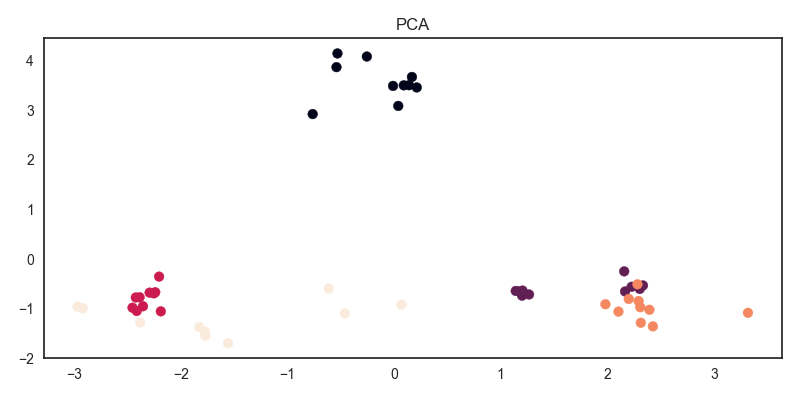
\includegraphics[width=\textwidth]{pca.png}
    \caption{Resultado de aplicar PCA para reducir a dos las dimensiones de los MFCC de un conjunto de sonidos de 5 especies animales.}
    \label{img:pca}
\end{figure}


\section{Manifold Learning}\label{sec:manifoldLearning}
El análisis de componentes principales no produce resultados de calidad si la relación entre las variables aleatorias es no lineal.
Los algoritmos de \textit{manifold learning} convierten los conjuntos de datos en otros de menor dimensionalidad conocidos como \textbf{manifolds}, obtenidos aplicando transformaciones no lineales sobre el espacio original de estos.

A continuación se mencionan algunos de los algoritmos de manifold learning más conocidos.

\subsection{Multi-dimensional Scaling}\label{subsec:MDS}

\textit{Multi-dimensional scaling} (MDS) es una técnica que tiene como objetivo obtener una representación del conjunto de datos en un espacio de menos dimensiones, preservando las distancias existentes entre los elementos en el espacio original.

En otras palabras, se busca minimizar la siguiente función objetivo:

\begin{equation}
    \label{eq:MDS}
    \sum_{i=1}^{N}\sum_{j=i+1}^{N}{d_{ij} - \hat{d}_{ij}}
\end{equation}

\noindent
dado un conjunto de datos de $N$ elementos, donde $d_{ij}$ y $\hat{d}_{ij}$ son las distancias entre los elementos $i$ y $j$ en los espacios original y reducido respectivamente.

Puesto que MDS se basa en las distancias entre los elementos y no utiliza la representación vectorial de estos, esta técnica puede emplearse incluso en casos en los que el conjunto de datos no posee tal representación (por ejemplo, cadenas de texto), siempre que la distancia o similitud entre ellos haya sido definida.

\subsection{Isomap}\label{subsec:isomap}

Al igual que PCA, MDS tampoco produce buenos resultados cuando la relación entre los puntos no es lineal.
Isomap puede considerarse como una extensión de MDS, desarrollada para procesar ese tipo de conjuntos de datos; y que a diferencia de MDS, se basa en la distancia \textit{geodésica} entre los puntos.

Para ello se construye un grafo donde existirá una arista entre los puntos $i$ y $j$ si estos son \textit{vecinos} en el espacio original, que tendrá un peso igual a la distancia euclidiana entre los puntos.

Luego la distancia geodésica entre cualquier par de puntos se corresponderá con el camino de costo mínimo entre estos en el grafo.
Finalmente, empleando esta nueva distancia, se aplica MDS\@.

El modo en que se determina si dos puntos son vecinos entre sí, está sujeto a variaciones.
Generalmente suele definirse un cierto radio para el que si dos puntos se encuentran a una distancia menor que este, se consideran vecinos.
Otro enfoque comúnmente empleado es el de, dado un valor $k$, fijar como vecinos de un punto los $k$ puntos más próximos a este.

\subsection{Locally Linear Embedding}\label{subsec:LLE}

Locally Linear Embedding (LLE) es una técnica para la reducción de dimensiones basada en la idea de analizar regiones locales de puntos superpuestas, para determinar la estructura local de los datos.

El primer paso del algoritmo consiste en hallar los puntos más cercanos a cada punto $x_i$, expresando luego a $x_i$ como una combinación lineal de estos.
De modo que se cumpla que $x_i =\sum_j {w_{ij}x_j}$, donde $\sum_j w_{ij}=1$ y $w_{ij} = 0$ si $x_j$ no es un vecino cercano de $x_i$.
La matriz de pesos $W$, de coeficientes $w_{ij}$ es encontrada minimizando el error cuadrático medio, dado por la ecuación:

\begin{equation}
    error(W) = \sum_i \left( x_i - \sum_j {w_{ij}x_j} \right)^2
\end{equation}

Luego, la reducción de dimensiones se realiza a partir de la matriz $W$ y un número de dimensiones $p$ prefijado.
Para ello, si $y_i$ es el vector correspondiente a $x_i$ en el nuevo espacio, y $Y$ matriz que tiene a los vectores $y_i$ como filas;
entonces se busca $Y$ tal que minimice la siguiente expresión:

\begin{equation}
    error(Y) = \sum_i \left( y_i - \sum_j {w_{ij}y_j} \right)^2
\end{equation}

Es decir, la nueva representación del conjunto de datos minimiza el error cuadrático medio a partir de los pesos encontrados para la representación original.
